\documentclass[preprint, 3p,
authoryear]{elsarticle} %review=doublespace preprint=single 5p=2 column
%%% Begin My package additions %%%%%%%%%%%%%%%%%%%

\usepackage[hyphens]{url}

  \journal{Systematic Reviews} % Sets Journal name

\usepackage{graphicx}
%%%%%%%%%%%%%%%% end my additions to header

\usepackage[T1]{fontenc}
\usepackage{lmodern}
\usepackage{amssymb,amsmath}
% TODO: Currently lineno needs to be loaded after amsmath because of conflict
% https://github.com/latex-lineno/lineno/issues/5
\usepackage{lineno} % add
\usepackage{ifxetex,ifluatex}
\usepackage{fixltx2e} % provides \textsubscript
% use upquote if available, for straight quotes in verbatim environments
\IfFileExists{upquote.sty}{\usepackage{upquote}}{}
\ifnum 0\ifxetex 1\fi\ifluatex 1\fi=0 % if pdftex
  \usepackage[utf8]{inputenc}
\else % if luatex or xelatex
  \usepackage{fontspec}
  \ifxetex
    \usepackage{xltxtra,xunicode}
  \fi
  \defaultfontfeatures{Mapping=tex-text,Scale=MatchLowercase}
  \newcommand{\euro}{€}
\fi
% use microtype if available
\IfFileExists{microtype.sty}{\usepackage{microtype}}{}
\usepackage[]{natbib}
\bibliographystyle{apalike}

\ifxetex
  \usepackage[setpagesize=false, % page size defined by xetex
              unicode=false, % unicode breaks when used with xetex
              xetex]{hyperref}
\else
  \usepackage[unicode=true]{hyperref}
\fi
\hypersetup{breaklinks=true,
            bookmarks=true,
            pdfauthor={},
            pdftitle={FACULTY OF ENGINEERING, DESIGN AND TECHNOLOGY DEPARTMENT OF COMPUTING AND TECHNOLOGY EASTER 2025 SEMESTER EXAMINATION - DATA SCIENCE LIFE CYCLE FINAL EXAMS},
            colorlinks=false,
            urlcolor=blue,
            linkcolor=magenta,
            pdfborder={0 0 0}}

\setcounter{secnumdepth}{5}
% Pandoc toggle for numbering sections (defaults to be off)


% tightlist command for lists without linebreak
\providecommand{\tightlist}{%
  \setlength{\itemsep}{0pt}\setlength{\parskip}{0pt}}







\begin{document}


\begin{frontmatter}

  \title{FACULTY OF ENGINEERING, DESIGN AND TECHNOLOGY DEPARTMENT OF
COMPUTING AND TECHNOLOGY EASTER 2025 SEMESTER EXAMINATION - DATA SCIENCE
LIFE CYCLE FINAL EXAMS}
    \author[Uganda Christian University]{Efprem Okello - J25M19/001,
Access Number - B31324%
  \corref{cor1}%
  }
   \ead{okelloefprem@gmail.com} 
      \affiliation[Uganda Christian University]{
    organization={Department of Computing and
Technology},addressline={P.O. Box 4},city={Kampala},country={Uganda},}
    \cortext[cor1]{Corresponding author}
  
  \begin{abstract}
  This report explores three key themes: Sentiment Analysis, AI in
  Education, and Financial Inclusion in East Africa, showcasing the
  power of data-driven insights to address modern challenges. Sentiment
  Analysis: Analyzes Amazon reviews to understand consumer emotions and
  preferences. Findings reveal balanced sentiments, highlighting product
  quality and usability, helping businesses improve customer
  relationships and products. AI in Education: Demonstrates how AI
  enhances higher education by analyzing student performance and
  improving assessments. Predictive models, like Logistic Regression,
  show AI's potential to boost academic success and teaching
  effectiveness. Financial Inclusion: Examines financial access in East
  Africa, where innovations like mobile money have expanded services.
  However, gaps remain for marginalized groups. Data analysis identifies
  digital payments and technology as key drivers, calling for targeted
  interventions to promote equity. In summary, this report highlights
  how data-driven approaches can transform understanding of human
  behavior, improve education, and advance financial inclusion, offering
  actionable insights for progress.
  \end{abstract}
    \begin{keyword}
    Sentiment Analysis \sep AI in Education \sep 
    Financial Inclusion
  \end{keyword}
  
 \end{frontmatter}

\section{Theme 2: Human Behaviour - Sentimental Analysis / Natural
Language processing of human text and
opinions}\label{theme-2-human-behaviour---sentimental-analysis-natural-language-processing-of-human-text-and-opinions}

\subsection{Introduction}\label{introduction}

The growth of digital content creation and social media has led to an
unprecedented increase in unstructured text data. Every day, people
express their thoughts and opinions through reviews, comments, and
feedback, generating vast amounts of user-generated content
\citep{liu2012sentiment}. This data holds valuable insights into human
emotions, preferences, and behaviors. Sentiment analysis has emerged as
a powerful tool for understanding these emotions
\citep{pang2008opinion}. By analyzing text, it helps uncover the
underlying feelings and thoughts people express. The ability to extract
sentiment from unstructured data provides meaningful insights, making it
indispensable for businesses, researchers, and anyone seeking to build a
deeper connection with their audience \citep{cambria2013new}.

As one of the world's largest e-commerce platforms, Amazon receives a
constant stream of customer feedback from product reviews to service
ratings \citep{hu2004mining}. This wealth of user-generated content
holds valuable insights into consumer sentiment, shedding light on what
people love, what frustrates them, and what they expect from their
shopping experiences. By applying Sentiment Analysis to Amazon's
customer feedback, we can uncover meaningful patterns in consumer
behavior \citep{zhang2018deep}. These insights go beyond just
understanding customer satisfaction and product preferences; they can
also reveal potential areas for improvement and even broader societal
trends, such as how online shopping impacts mental well-being and social
dynamics.

\subsection{Methodology}\label{methodology}

The analysis followed a structured approach, incorporating data
collection, preprocessing, exploratory analysis, and modeling to extract
insights from Amazon customer reviews.

\begin{itemize}
\item
  \textbf{Data Collection and Pre-processing:} Sentiment-labeled data
  set containing customer feedback was obtained from the UC Irvine
  Machine Learning Repository and imported into python for analysis. The
  text data underwent pre-processing, where it was converted to
  lowercase, special characters, stop-words, and short words were
  removed. This enhanced the relevance of the data and allowed for more
  accurate analysis.
\item
  \textbf{Exploratory Data Analysis:}In the exploratory data analysis
  phase, we examined the sentiment distribution, revealing an even split
  between positive and negative reviews. A word frequency analysis was
  conducted to identify key themes in customer feedback. Words such as
  ``phone,'' ``great,'' and ``good'' were frequently mentioned,
  highlighting common sentiments. A word cloud visualization was created
  to graphically represent the most common terms, focusing on product
  quality and usability.
\item
  \textbf{Sentiment Classification:} For sentiment classification, we
  applied TF-IDF vectorization to convert text data into numerical
  format. A Naïve Bayes classifier was then trained to predict
  sentiment, and the model was evaluated using accuracy scores,
  classification reports, and a confusion matrix. We also validated the
  model with hypothetical test samples, demonstrating its ability to
  predict sentiment.
\item
  \textbf{Unsupervised Learning (Clustering):} To provide an
  unsupervised perspective, we implemented K-Means clustering, grouping
  the reviews into two sentiment-based clusters. This clustering
  approach helped us explore sentiment trends in the data without
  predefined labels.
\end{itemize}

\subsection{Findings}\label{findings}

\subsubsection{Sentiment Distribution}\label{sentiment-distribution}

The sentiment analysis reveals a perfectly balanced distribution between
positive and negative feedback. Out of the total dataset, 500 reviews
(50\%) express negative sentiment (Sentiment = 0), while 500 reviews
(50\%) convey positive sentiment (Sentiment = 1). This even split
suggests a diverse range of customer experiences, with equal
representation of satisfaction and dissatisfaction.

\begin{center}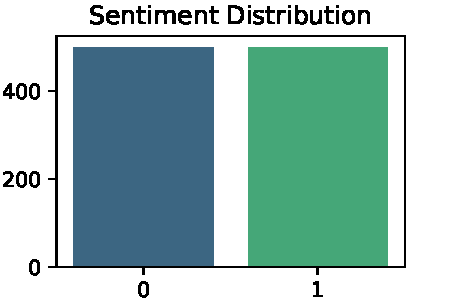
\includegraphics[width=0.7\linewidth]{Final-Report_files/figure-latex/unnamed-chunk-5-1} \end{center}

\subsubsection{Word Cloud Visualization}\label{word-cloud-visualization}

The text analysis reveals key themes in customer feedback, with
``phone'' being the most frequently mentioned word, appearing 168 times.
This suggests that many reviews focus on mobile devices, likely
discussing their performance, features, or overall satisfaction. The
words ``great'' (99) and ``good'' (77) indicate a generally positive
sentiment, implying that customers are largely satisfied with their
purchases. ``Product'' (55) and ``quality'' (49) further reinforce this,
highlighting that shoppers often comment on the overall value and
craftsmanship of their items. Specific mentions of ``headset'' (48),
``battery'' (46), and ``sound'' (43) suggest that many reviews relate to
audio devices, possibly wireless headphones or earphones. The frequent
appearance of ``works'' (47) implies that customers often evaluate
whether the product functions as expected. Additionally, ``use'' (41)
indicates that usability is an important factor in customer experiences.
Overall, the feedback suggests that customers are generally pleased with
the quality and performance of their purchases, particularly in relation
to phones and audio accessories.

\begin{verbatim}
## (-0.5, 799.5, 399.5, -0.5)
\end{verbatim}

\begin{center}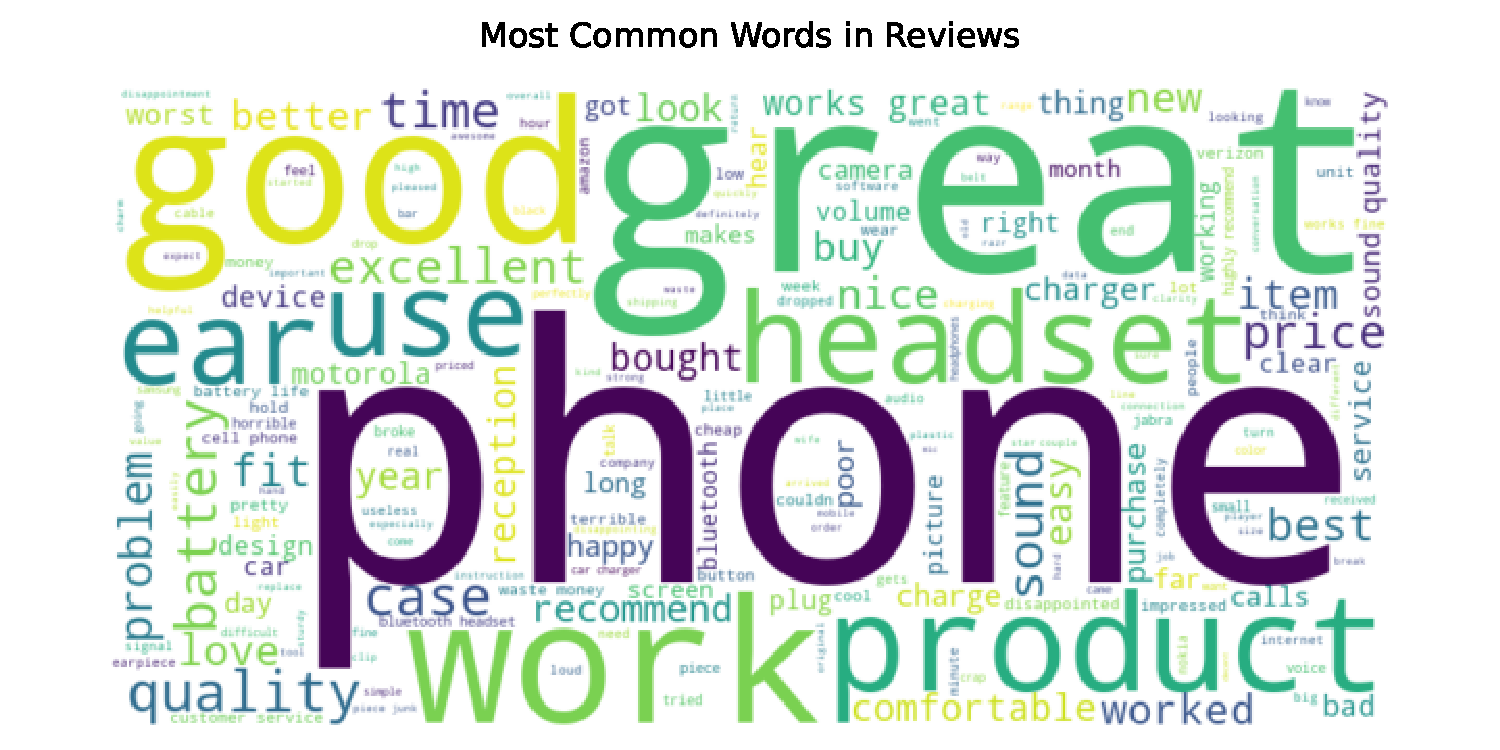
\includegraphics[width=0.7\linewidth]{Final-Report_files/figure-latex/unnamed-chunk-6-3} \end{center}

\subsection{Build, Evaluate and Optimize
models}\label{build-evaluate-and-optimize-models}

\paragraph{Model Evaluation}\label{model-evaluation}

The model demonstrates a solid performance with an overall accuracy of
81\%, correctly predicting the class in 81\% of the cases. It performs
well across both classes, with Class 1 showing slightly better results.
For Class 0, the model achieves a precision of 82\% and a recall of
75\%, indicating that it correctly identifies 82\% of the predicted
Class 0 instances, though it misses about 25\% of actual Class 0
instances. For Class 1, precision stands at 80\%, and recall is higher
at 86\%, meaning it identifies 86\% of the true Class 1 instances but
with a slightly lower precision. The F1-scores are balanced for both
classes, with 0.79 for Class 0 and 0.83 for Class 1, reflecting a strong
trade-off between precision and recall. The model's performance is
consistent across both classes, as indicated by the macro and weighted
averages of 81\% for precision, recall, and F1-score, showing a
well-rounded and effective classification model.

\begin{verbatim}
## MultinomialNB()
\end{verbatim}

\begin{verbatim}
## <string>:3: FutureWarning: DataFrame.applymap has been deprecated. Use DataFrame.map instead.
\end{verbatim}

\begin{verbatim}
## ==================================================
\end{verbatim}

\begin{verbatim}
## Model Evaluation Metrics
\end{verbatim}

\begin{verbatim}
## ==================================================
\end{verbatim}

\begin{verbatim}
## Accuracy Score: 0.81
\end{verbatim}

\begin{verbatim}
## Classification Report:
\end{verbatim}

\begin{verbatim}
## +--------------+-----------+--------+----------+---------+
## |              | precision | recall | f1-score | support |
## +--------------+-----------+--------+----------+---------+
## |      0       |   0.82    |  0.75  |   0.79   |  93.0   |
## |      1       |    0.8    |  0.86  |   0.83   |  107.0  |
## |   accuracy   |   0.81    |  0.81  |   0.81   |  0.81   |
## |  macro avg   |   0.81    |  0.81  |   0.81   |  200.0  |
## | weighted avg |   0.81    |  0.81  |   0.81   |  200.0  |
## +--------------+-----------+--------+----------+---------+
\end{verbatim}

\begin{verbatim}
## ==================================================
\end{verbatim}

\subparagraph{Confusion Matrix}\label{confusion-matrix}

The confusion matrix reveals how well the model predicts Negative and
Positive cases. The model correctly identified 70 Negative cases and 92
Positive cases. However, it incorrectly predicted 23 Negative cases as
Positive and 15 Positive cases as Negative. Overall, the model performs
well, but there is room for improvement, particularly in reducing the
number of False Positives and False Negatives.

\begin{center}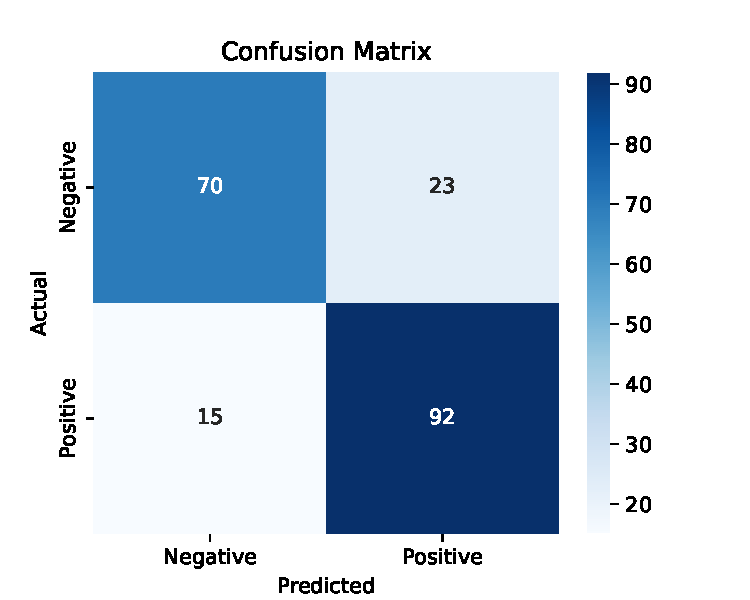
\includegraphics[width=0.7\linewidth]{Final-Report_files/figure-latex/unnamed-chunk-8-5} \end{center}

\newpage

\section{Theme 4: Education: Artificial Intelligence (AI) in Higher
Education}\label{theme-4-education-artificial-intelligence-ai-in-higher-education}

\subsection{Introduction}\label{introduction-1}

Education is a key driver of national development, and improving the
quality of higher education is essential for progress. One way to
achieve this is by using faster methods to assess student performance
and teaching effectiveness. Traditional assessment methods can be slow
and limited \citep{bennett2011formative}, but Artificial Intelligence
(AI) offers a promising solution \citep{luckin2016intelligence}. AI can
analyze large amounts of data quickly and identify patterns that can
help improve both teaching methods and student outcomes
\citep{baker2014educational}. In higher education, machine learning
algorithms, a type of AI, can be used to classify student performance
and evaluate teaching approaches. By analyzing data from student
assessments and other academic activities, these algorithms can provide
valuable insights. The goal of this study is to find the most effective
approach for improving student performance.

\subsection{Methodology}\label{methodology-1}

This study aims to predict student performance, specifically determining
whether a student will pass or fail based on various factors. The
process involved several key steps, including data collection,
preprocessing, exploratory analysis, model building, evaluation, and
validation.

\begin{itemize}
\item
  \textbf{Data Collection and Preprocessing:} The dataset used in the
  study contains various student characteristics such as their previous
  grades, study time, age, and alcohol consumption (both on weekdays and
  weekends). In the preprocessing stage, categorical variables like
  whether a student wants to pursue higher education were converted into
  numeric values using label encoding. Additionally, the target
  variable, the final grade (denoted as G3), was transformed into a
  binary classification problem. If a student's final grade was 10 or
  more, they were considered to have ``passed'' (label 1), while those
  with grades below 10 were categorized as ``fail'' (label 0).
\item
  \textbf{Exploratory Data Analysis:} Following preprocessing, an
  in-depth analysis of the data was conducted to understand the
  relationships between different variables and their impact on student
  performance. Histograms and box plots were created to visually examine
  the distribution of grades and to highlight the study time's influence
  on the final grade. A correlation matrix was also generated to
  identify the factors most closely related to student performance. This
  analysis revealed that previous grades and study time were the most
  significant predictors of final performance.
\item
  \textbf{Model Building:} In the next phase, various features were
  selected for use in the predictive model. The selected features
  included previous grades, weekly study time, the number of past class
  failures, and other factors like age, and alcohol consumption. The
  dataset was split into training and testing sets to ensure an unbiased
  evaluation of the models. Three different machine learning algorithms
  were applied: Logistic Regression, Random Forest, and Gradient
  Boosting. These models were trained using the training dataset, and
  their performance was evaluated on the testing set.
\item
  \textbf{Model Evaluation:} The models were evaluated based on their
  accuracy, precision, recall, and F1-score. Logistic Regression
  provided the best overall performance, as it showed the highest
  accuracy in predicting whether a student would pass or fail. Random
  Forest and Gradient Boosting also performed well but did not
  outperform Logistic Regression in this study. Based on these results,
  Logistic Regression was selected as the best model for predicting
  student performance.
\item
  \textbf{Validation:} To validate the effectiveness of the model, a
  sample student's data was used to predict their final grade. The
  student's characteristics---such as age, study time, and alcohol
  consumption---were input into the trained Logistic Regression model,
  which predicted whether they would pass or fail. This validation step
  confirmed the model's capability to make accurate predictions based on
  the input features.
\end{itemize}

\subsection{Findings}\label{findings-1}

\subsubsection{Historical student
performance}\label{historical-student-performance}

The distribution of final grades (G3) reveals that most students pass
their final exams.Out of 649 students, 549 (84.6\%) passed and 100
(15.4\%) failed, indicating a generally high pass rate.

\begin{center}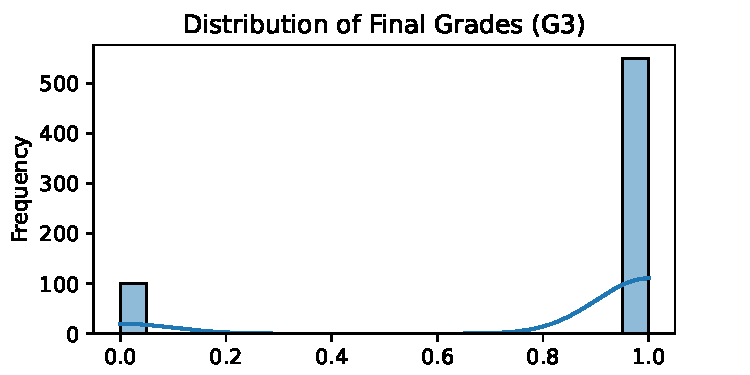
\includegraphics[width=0.7\linewidth]{Final-Report_files/figure-latex/unnamed-chunk-10-7} \end{center}

\subsubsection{Average study time vs Final
Grade}\label{average-study-time-vs-final-grade}

The average study time for students reveals a notable difference between
those who passed and those who failed. Students who passed (G3 = 1)
spent an average of 1.99 hours per week studying, while those who failed
(G3 = 0) averaged only 1.61 hours per week. This indicates a positive
correlation between study time and academic performance, suggesting that
increased study time contributes to better outcomes.

\begin{center}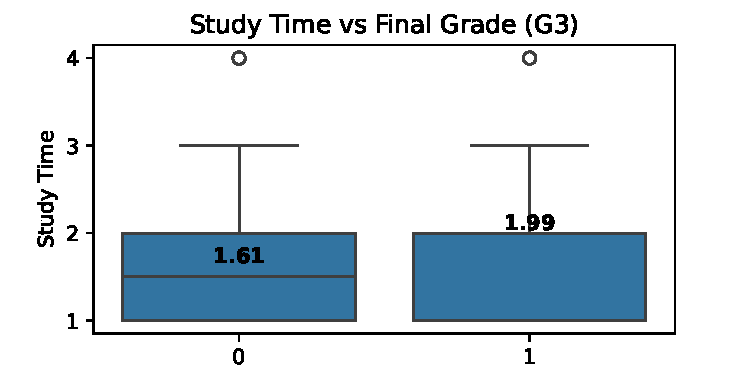
\includegraphics[width=0.7\linewidth]{Final-Report_files/figure-latex/unnamed-chunk-11-9} \end{center}

\subsubsection{Predictors of Final
Grade}\label{predictors-of-final-grade}

The correlation analysis reveals that the strongest predictors of final
grades (G3) are early academic performance (G1 and G2) and aspirations
for higher education (higher), both showing significant positive
correlations. Moderate positive correlations exist for study time and
parental education, suggesting their supportive role in academic
success. Conversely, past failures, alcohol consumption, and absences
have strong negative correlations, indicating they are major barriers to
performance. Factors like family support, extracurricular activities,
and guardian type have minimal impact on grades.

\begin{verbatim}
## (array([0.5]), [Text(0.5, 0, 'G3')])
\end{verbatim}

\begin{center}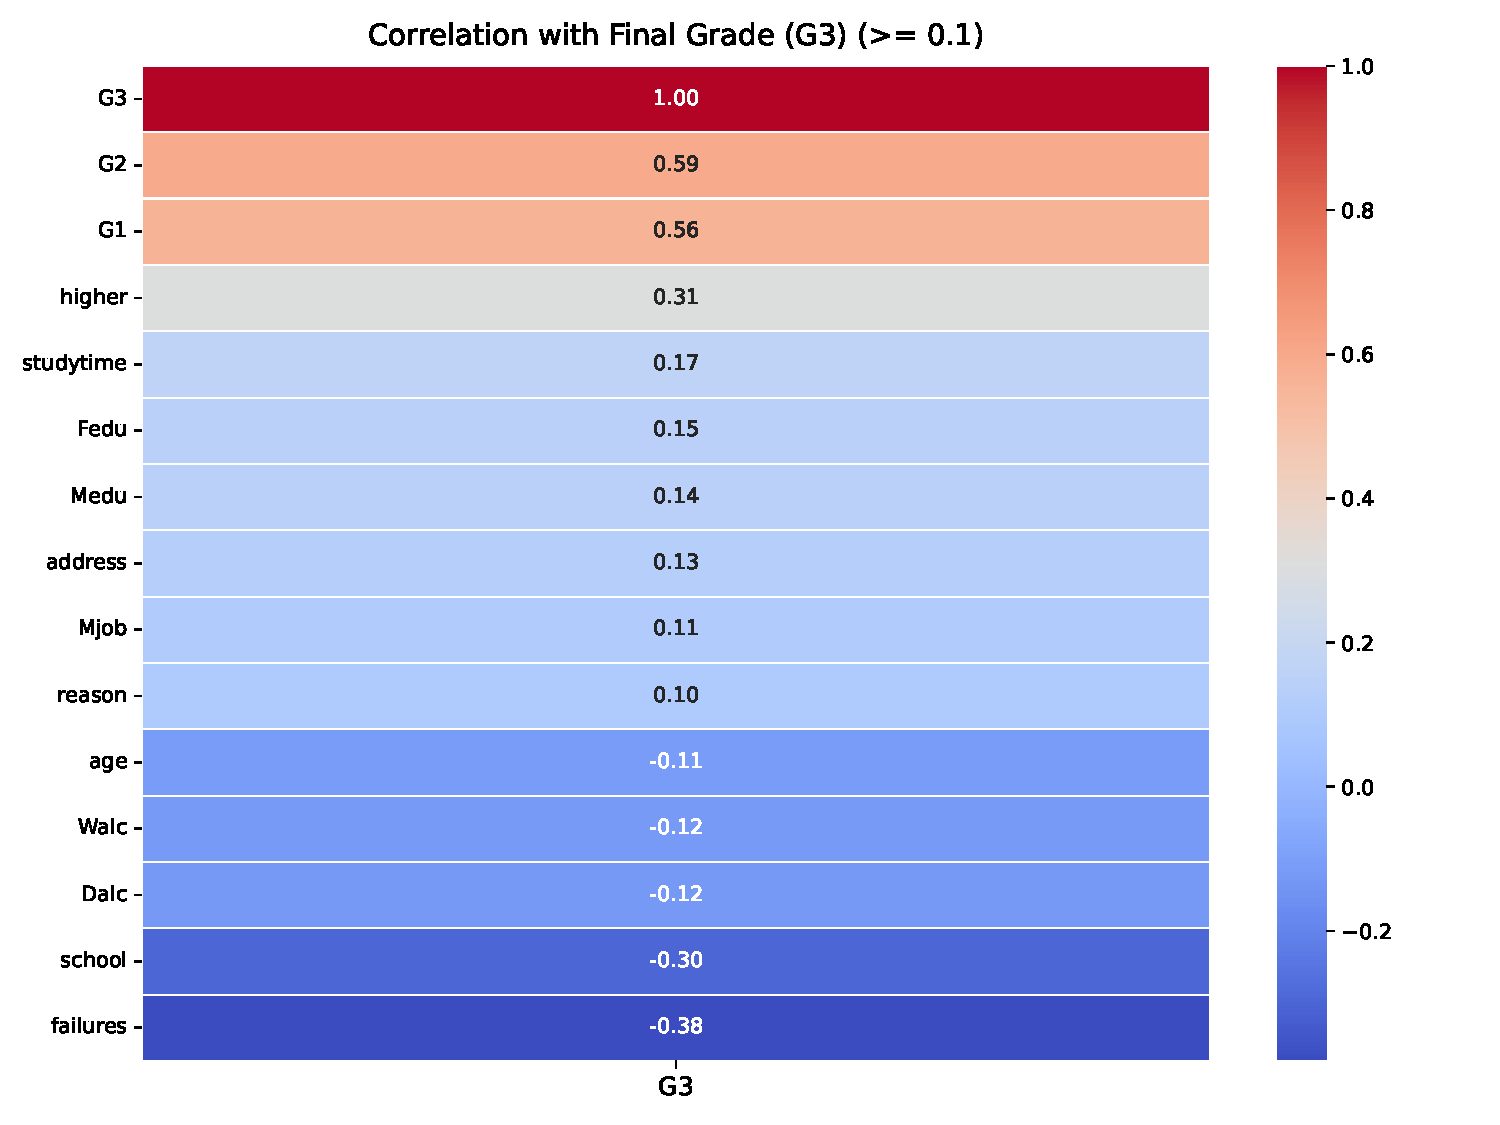
\includegraphics[width=0.7\linewidth]{Final-Report_files/figure-latex/unnamed-chunk-12-11} \end{center}

\subsubsection{Selected Models}\label{selected-models}

\paragraph{Model 1: Logistic
Regression}\label{model-1-logistic-regression}

\hfill\break
The logistic regression model achieved an overall accuracy of 89.2\%.
The model performs exceptionally well in predicting class 1, with a
precision of 92\%, a recall of 97\%, and an F1-score of 94\%, based on
115 instances. However, its performance in predicting class 0 is weaker,
with a precision of 56\%, a recall of 33\%, and an F1-score of 42\%,
based on 15 instances. The macro average F1-score is 68\%, reflecting
the imbalance in class performance, while the weighted average F1-score
of 88\% indicates strong overall predictive capability.

\begin{verbatim}
## LogisticRegression(random_state=42)
\end{verbatim}

\begin{verbatim}
## <string>:3: FutureWarning: DataFrame.applymap has been deprecated. Use DataFrame.map instead.
\end{verbatim}

\begin{verbatim}
## ==================================================
\end{verbatim}

\begin{verbatim}
## Logistic Regression Evaluation Metrics
\end{verbatim}

\begin{verbatim}
## ==================================================
\end{verbatim}

\begin{verbatim}
## Accuracy Score: 0.89
\end{verbatim}

\begin{verbatim}
## Classification Report:
\end{verbatim}

\begin{verbatim}
## +--------------+-----------+--------+----------+---------+
## |              | precision | recall | f1-score | support |
## +--------------+-----------+--------+----------+---------+
## |      0       |   0.56    |  0.33  |   0.42   |  15.0   |
## |      1       |   0.92    |  0.97  |   0.94   |  115.0  |
## |   accuracy   |   0.89    |  0.89  |   0.89   |  0.89   |
## |  macro avg   |   0.74    |  0.65  |   0.68   |  130.0  |
## | weighted avg |   0.88    |  0.89  |   0.88   |  130.0  |
## +--------------+-----------+--------+----------+---------+
\end{verbatim}

\begin{verbatim}
## ==================================================
\end{verbatim}

\paragraph{Model 2: Random Forest
Classifier}\label{model-2-random-forest-classifier}

\hfill\break
The Random Forest model achieved an overall accuracy of 84.6\%. The
model performs well in predicting class 1, with a precision of 91\%, a
recall of 92\%, and an F1-score of 91\%, based on 115 instances.
However, its performance in predicting class 0 is considerably lower,
with a precision of 31\%, a recall of 27\%, and an F1-score of 29\%,
based on 15 instances. The macro average F1-score of 60\% highlights
this class imbalance, while the weighted average F1-score of 84\%
suggests strong overall predictive ability, driven mainly by class 1
performance.

\begin{verbatim}
## RandomForestClassifier(random_state=42)
\end{verbatim}

\begin{verbatim}
## <string>:3: FutureWarning: DataFrame.applymap has been deprecated. Use DataFrame.map instead.
\end{verbatim}

\begin{verbatim}
## ==================================================
\end{verbatim}

\begin{verbatim}
## Random Forest Evaluation Metrics
\end{verbatim}

\begin{verbatim}
## ==================================================
\end{verbatim}

\begin{verbatim}
## Accuracy Score: 0.85
\end{verbatim}

\begin{verbatim}
## Classification Report:
\end{verbatim}

\begin{verbatim}
## +--------------+-----------+--------+----------+---------+
## |              | precision | recall | f1-score | support |
## +--------------+-----------+--------+----------+---------+
## |      0       |   0.31    |  0.27  |   0.29   |  15.0   |
## |      1       |   0.91    |  0.92  |   0.91   |  115.0  |
## |   accuracy   |   0.85    |  0.85  |   0.85   |  0.85   |
## |  macro avg   |   0.61    |  0.59  |   0.6    |  130.0  |
## | weighted avg |   0.84    |  0.85  |   0.84   |  130.0  |
## +--------------+-----------+--------+----------+---------+
\end{verbatim}

\begin{verbatim}
## ==================================================
\end{verbatim}

\paragraph{Model 3: Gradient Boosting
Classifier}\label{model-3-gradient-boosting-classifier}

\hfill\break
The Gradient Boosting model achieved an overall accuracy of 85.4\%. It
performed well in predicting class 1, with a precision of 92\%, a recall
of 91\%, and an F1-score of 92\%, based on 115 instances. For class 0,
the model showed moderate performance, with a precision of 38\%, a
recall of 40\%, and an F1-score of 39\%, based on 15 instances. The
macro average F1-score of 65\% reflects this disparity, while the
weighted average F1-score of 86\% indicates that the model maintains
strong overall predictive performance, primarily driven by class 1.

\begin{verbatim}
## GradientBoostingClassifier(random_state=42)
\end{verbatim}

\begin{verbatim}
## <string>:3: FutureWarning: DataFrame.applymap has been deprecated. Use DataFrame.map instead.
\end{verbatim}

\begin{verbatim}
## ==================================================
\end{verbatim}

\begin{verbatim}
## Gradient Boosting Evaluation Metrics
\end{verbatim}

\begin{verbatim}
## ==================================================
\end{verbatim}

\begin{verbatim}
## Accuracy Score: 0.85
\end{verbatim}

\begin{verbatim}
## Classification Report:
\end{verbatim}

\begin{verbatim}
## +--------------+-----------+--------+----------+---------+
## |              | precision | recall | f1-score | support |
## +--------------+-----------+--------+----------+---------+
## |      0       |   0.38    |  0.4   |   0.39   |  15.0   |
## |      1       |   0.92    |  0.91  |   0.92   |  115.0  |
## |   accuracy   |   0.85    |  0.85  |   0.85   |  0.85   |
## |  macro avg   |   0.65    |  0.66  |   0.65   |  130.0  |
## | weighted avg |   0.86    |  0.85  |   0.86   |  130.0  |
## +--------------+-----------+--------+----------+---------+
\end{verbatim}

\begin{verbatim}
## ==================================================
\end{verbatim}

\paragraph{Model performance
comparison}\label{model-performance-comparison}

\hfill\break
The Logistic Regression model is the recommended choice, achieving the
highest accuracy of 89.2\%. It demonstrated strong performance in
predicting class 1, with a precision of 92\%, a recall of 97\%, and an
F1-score of 94\%, based on 115 instances. Although its performance for
class 0 was lower (precision: 56\%, recall: 33\%, F1-score: 42\% for 15
instances), the overall weighted F1-score of 88\% indicates robust
predictive ability. Given its superior accuracy and balanced
performance, Logistic Regression is the most reliable model for this
classification task.

\begin{verbatim}
## 
## Recommended Model: Logistic Regression Results with Accuracy: 0.8923076923076924
\end{verbatim}

\subsubsection{Model Validation}\label{model-validation}

For a 31-year-old student who studies 5 to 10 hours per week, has no
record of past failures, aspires to pursue higher education, and
consumes alcohol once on weekdays and twice on weekends, the trained
Logistic Regression model predicted a pass. This outcome aligns with
expectations, as the student's consistent study habits, lack of academic
failures, and motivation for higher education are strong indicators of
academic success.

\begin{verbatim}
## Predicted Final Grade (G3) for the student: 1
\end{verbatim}

\section{Theme 3: : Finance- Financial Access and
Inclusion}\label{theme-3-finance--financial-access-and-inclusion}

\subsection{Introduction}\label{introduction-2}

Financial access and inclusion are critical drivers of economic growth
and poverty reduction. Across Africa, the expansion of credit, funding
opportunities, and digital financial platforms---such as mobile
money---has significantly improved financial access
\citep{suri2016long}. These innovations have facilitated transactions,
savings, and credit acquisition for millions, promoting financial
empowerment and economic participation. However, despite these
advancements, financial inclusion remains uneven, with marginalized
groups such as women, the elderly, and rural populations facing
persistent barriers to access \citep{allen2016african}. Socioeconomic
disparities, limited financial literacy, inadequate infrastructure, and
restrictive financial policies contribute to their exclusion, limiting
their ability to fully benefit from financial services. This analysis
seeks to examine financial access and service usage data to identify
existing gaps and inequalities. By understanding these disparities,
targeted interventions can be proposed to enhance inclusivity and ensure
that financial systems cater to all, fostering equitable economic
development.

\subsection{Methodology}\label{methodology-2}

The methodology employed in this analysis is designed to comprehensively
evaluate financial inclusion across East African countries (Burundi,
Kenya, Rwanda, Tanzania, and Uganda) using a structured, data-driven
approach.

\begin{itemize}
\item
  \textbf{Data Preparation:} The analysis began with loading the dataset
  (DatabankWide.xlsx) and selecting relevant variables that capture key
  dimensions of financial inclusion, such as account ownership, access
  to financial services, usage patterns, and socio-economic dynamics.
  The dataset is filtered to focus on East African countries, ensuring
  the analysis is region-specific. Missing values are addressed using a
  systematic imputation strategy: numeric variables are filled with the
  mean or median (depending on skewness), while categorical variables
  are filled with the mode. This ensures the dataset is complete and
  ready for analysis. To handle categorical variables, a combination of
  Label Encoding and One-Hot Encoding were applied.
\item
  \textbf{Exploratory Data Analysis (EDA):}The EDA phase focused on
  understanding the relationships between variables and identifying key
  drivers of financial inclusion. A correlation analysis was conducted
  to determine which variables have the strongest association with the
  Financial Inclusion Index (FII). Variables with a correlation
  coefficient of 0.5 or higher were identified as significant
  contributors to financial inclusion. Visualizations, such as heatmaps
  and box plots, were used to explore the distribution of financial
  service usage and access across different demographics (e.g., gender,
  labor force status) and socio-economic dynamics (e.g., digital
  payments, savings behavior).
\item
  \textbf{Feature Engineering:} To quantify financial inclusion, a
  Financial Inclusion Index (FII) was constructed using weighted scores
  for three dimensions:
\end{itemize}

\begin{enumerate}
\def\labelenumi{\roman{enumi}.}
\tightlist
\item
  \textbf{Ownership:} To measure account and card ownership.
\item
  \textbf{Access:} As proxies of access to financial services using
  account and card ownership data.
\item
  \textbf{Usage:} To evaluates the active use of financial services,
  such as making deposits or using debit/credit cards.
\end{enumerate}

Each dimension was weighted (ownership: 40\%, access: 30\%, usage: 30\%)
to reflect its relative importance. The FII was then calculated as a
composite score scaled to 0--100, providing a standardized metric for
comparing financial inclusion across countries and demographics.

\begin{itemize}
\item
  \textbf{Predictive Modeling:} The analysis employs machine learning to
  predict the Financial Inclusion Index based on the identified
  significant variables. Five regression models are evaluated: Linear
  Regression, Random Forest Regressor, Gradient Boosting Regressor,
  Support Vector Regressor (SVR), K-Nearest Neighbors Regressor (KNN).
  Each model was trained on 80\% of the data and evaluated on the
  remaining 20\%. Performance metrics such as Mean Absolute Error (MAE),
  Mean Squared Error (MSE), and R-squared (R²) were used to compare the
  models. The Linear Regression model was selected for further
  validation due to its interpretability and competitive performance.
\item
  \textbf{Model Evaluation and Interpretation:} The Linear Regression
  model was validated using 5-fold cross-validation to confirms its
  consistency across different subsets of the data. The model's
  coefficients were interpreted to understand the impact of each feature
  on the Financial Inclusion Index. For example: Positive coefficients
  indicate that higher values of the feature (e.g., digital payments,
  savings behavior) are associated with increased financial inclusion.
  Negative coefficients suggest that certain factors (e.g., inactive
  accounts) may hinder financial inclusion. Finally, the model was used
  to make predictions on the test set, and its performance is evaluated
  using MAE, MSE, and R². The results demonstrate that the model
  provides a reliable estimate of financial inclusion, with an R² value
  indicating a strong fit to the data.
\end{itemize}

\subsection{Summary of Findings}\label{summary-of-findings}

\subsubsection{Identification of variables that affect financial
inclusion}\label{identification-of-variables-that-affect-financial-inclusion}

The correlation analysis reveals that digital payments, savings
behavior, and mobile money usage are the strongest drivers of financial
inclusion, with correlations exceeding 0.85. Urban populations and
individuals in the labor force show higher financial inclusion compared
to rural and out-of-labor-force groups. Access to technology, such as
mobile phones and the internet, also plays a significant role, with
correlations above 0.70. Gender-specific analysis indicates that women
and men exhibit similar trends, though women show slightly stronger
correlations in areas like saving for education or old age.

\begin{verbatim}
## (array([0.5]), [Text(0.5, 0, 'financial_inclusion_index')])
\end{verbatim}

\begin{center}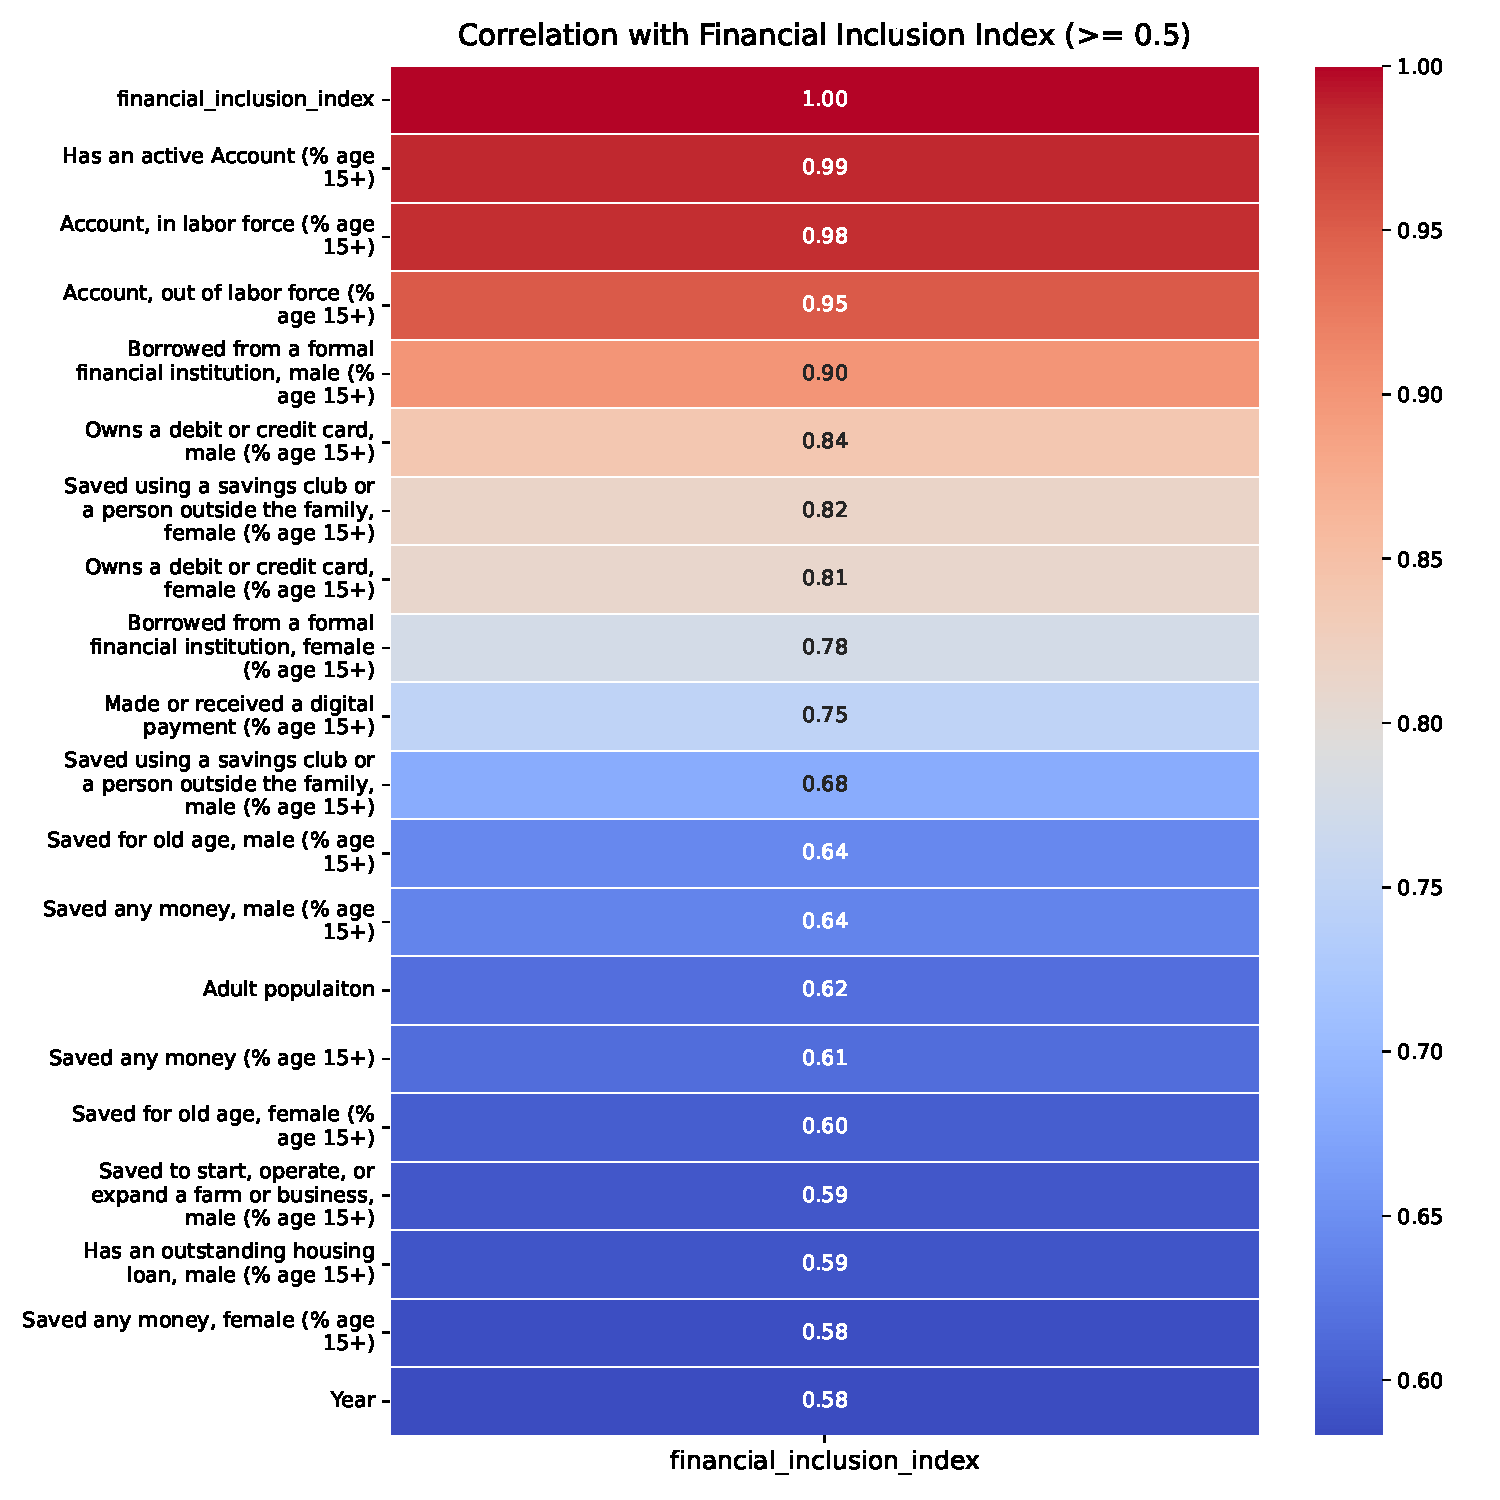
\includegraphics[width=0.8\linewidth]{Final-Report_files/figure-latex/unnamed-chunk-20-13} \end{center}

\subsubsection{Financial Service-Usage/Access Distribution Across
Population
Demographics}\label{financial-service-usageaccess-distribution-across-population-demographics}

The analysis shows that less than half of people aged 15+ actively use
financial accounts (median: 43.34\%). Those in the labor force have
higher account ownership (median: 49.85\%) compared to those not working
(median: 30.03\%), highlighting the impact of employment on financial
access. Men are more likely to borrow from formal institutions (median:
10.02\%) and own debit/credit cards (median: 16.39\%) than women
(borrowing: median 6.87\%; card ownership: median 10.74\%).

\begin{verbatim}
## ([<matplotlib.axis.XTick object at 0x000002146564AD50>, <matplotlib.axis.XTick object at 0x0000021461050310>, <matplotlib.axis.XTick object at 0x00000214601D3610>, <matplotlib.axis.XTick object at 0x00000214655CF7D0>, <matplotlib.axis.XTick object at 0x000002145D722090>, <matplotlib.axis.XTick object at 0x000002145D723390>, <matplotlib.axis.XTick object at 0x000002145D719050>], [Text(0, 0, 'Has an active\nAccount (% age 15+)'), Text(1, 0, 'Account, in labor\nforce (% age 15+)'), Text(2, 0, 'Account, out of\nlabor force (% age\n15+)'), Text(3, 0, 'Borrowed from a\nformal financial\ninstitution, male (%\nage 15+)'), Text(4, 0, 'Owns a debit or\ncredit card, male (%\nage 15+)'), Text(5, 0, 'Borrowed from a\nformal financial\ninstitution, female\n(% age 15+)'), Text(6, 0, 'Owns a debit or\ncredit card, female\n(% age 15+)')])
\end{verbatim}

\begin{center}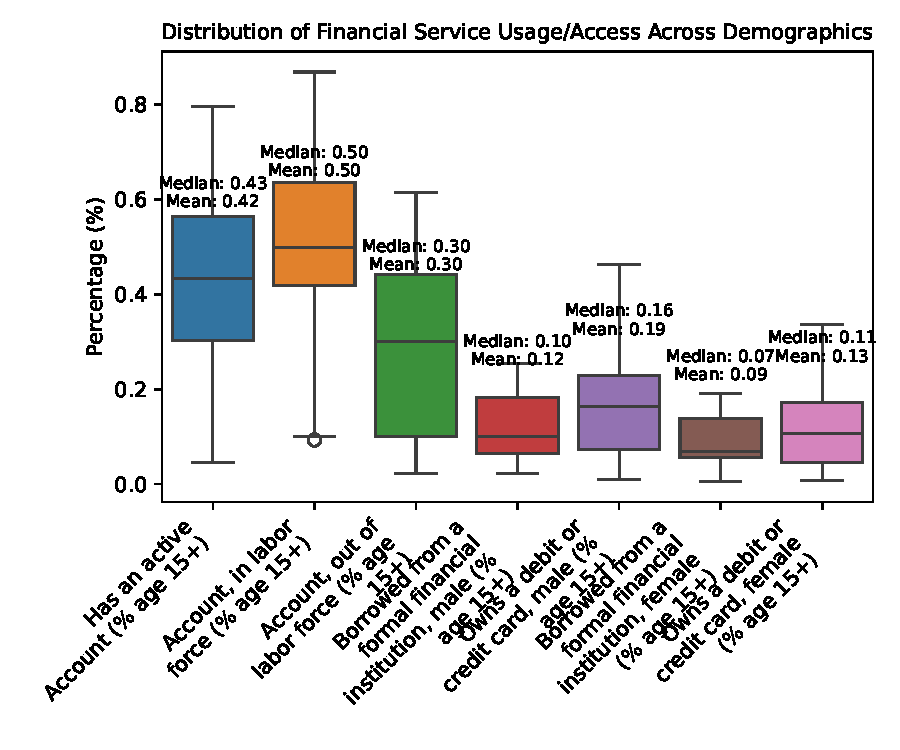
\includegraphics[width=0.9\linewidth]{Final-Report_files/figure-latex/unnamed-chunk-22-15} \end{center}

\subsubsection{Financial Service-Usage/Access Distribution Across
Socio-Economic
Dynamics}\label{financial-service-usageaccess-distribution-across-socio-economic-dynamics}

The analysis of socio-economic dynamics reveals that digital payments
are widely adopted, with a median of 48.64\% of individuals aged 15+
having made or received digital payments, matching the mean of 48.64\%.
This indicates a balanced distribution and highlights the growing role
of digital financial services in promoting inclusion. On the other hand,
savings through informal channels, such as savings clubs or individuals
outside the family, is less common among women, with a median of 23.59\%
and a mean of 24.40\%. This suggests that while digital payments are
becoming mainstream, informal savings mechanisms remain a secondary
option for many women.

\begin{verbatim}
## ([<matplotlib.axis.XTick object at 0x000002145D722D50>, <matplotlib.axis.XTick object at 0x00000214602264D0>], [Text(0, 0, 'Made or received a\ndigital payment (%\nage 15+)'), Text(1, 0, 'Saved using a\nsavings club or a\nperson outside the\nfamily, female (%\nage 15+)')])
\end{verbatim}

\begin{center}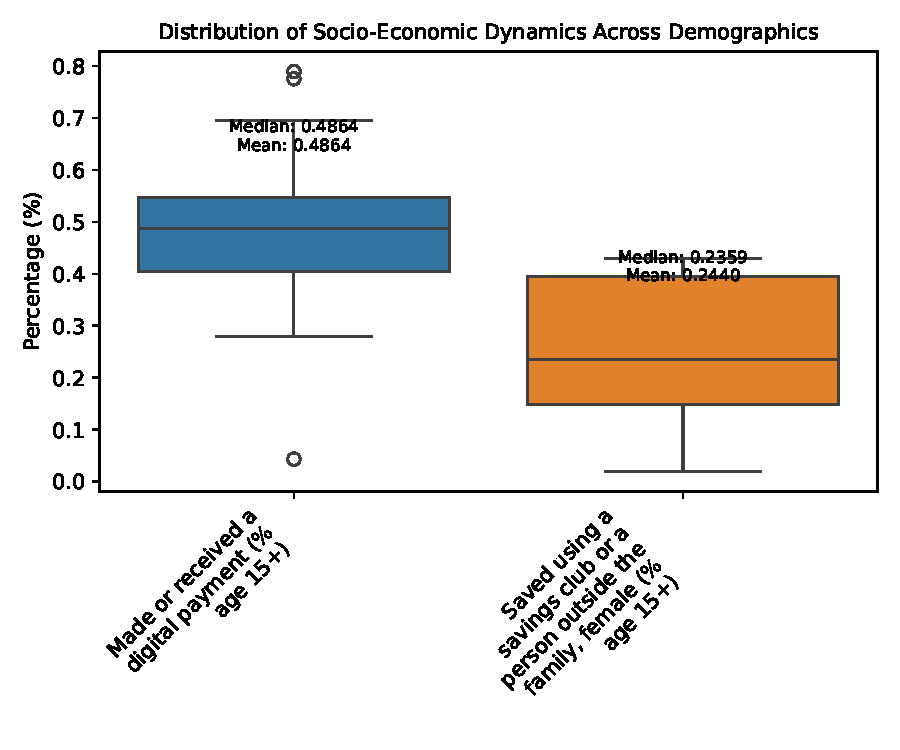
\includegraphics[width=0.9\linewidth]{Final-Report_files/figure-latex/unnamed-chunk-23-17} \end{center}

\subsubsection{Identify Gaps in Financial Service-Usage/Access
(Marginalized
Groups)}\label{identify-gaps-in-financial-service-usageaccess-marginalized-groups}

The analysis of financial service usage and access among marginalized
groups reveals notable disparities between men and women. On average,
men are more likely to borrow from formal financial institutions (mean:
12.06\%) and own debit/credit cards (mean: 18.67\%) compared to women
(borrowing: mean 8.83\%; card ownership: mean 12.79\%). These gaps
highlight significant gender-based inequalities in access to formal
financial services.

\begin{verbatim}
## ([<matplotlib.axis.XTick object at 0x0000021465648A90>, <matplotlib.axis.XTick object at 0x0000021465652210>, <matplotlib.axis.XTick object at 0x000002146648AB90>, <matplotlib.axis.XTick object at 0x0000021465667690>], [Text(0, 0, 'Borrowed from a\nformal financial\ninstitution, male (%\nage 15+)'), Text(1, 0, 'Borrowed from a\nformal financial\ninstitution, female\n(% age 15+)'), Text(2, 0, 'Owns a debit or\ncredit card, male (%\nage 15+)'), Text(3, 0, 'Owns a debit or\ncredit card, female\n(% age 15+)')])
\end{verbatim}

\begin{center}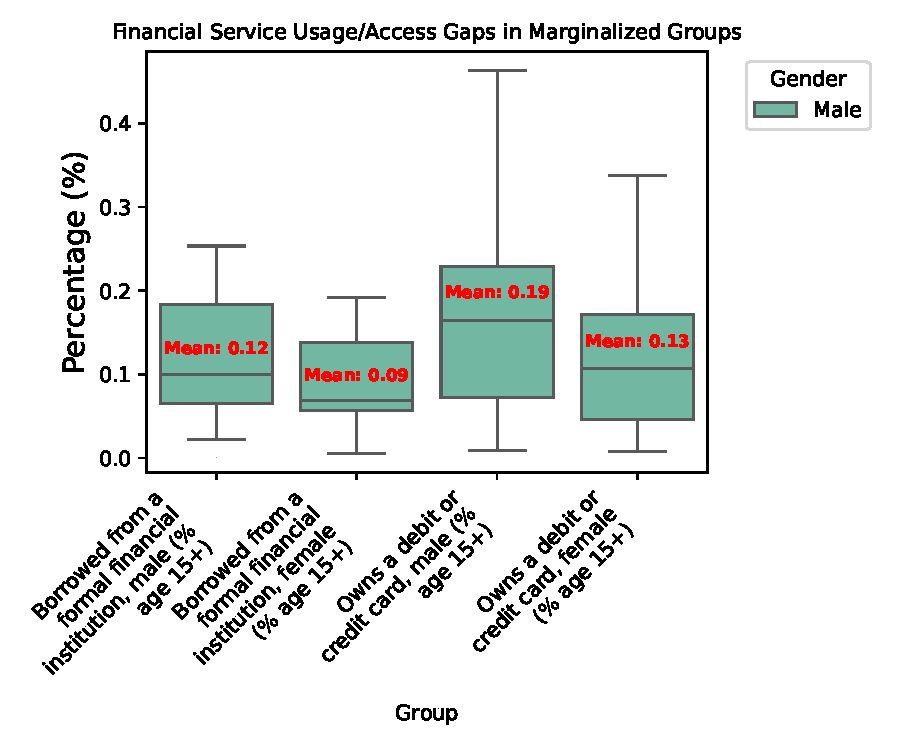
\includegraphics[width=0.9\linewidth]{Final-Report_files/figure-latex/unnamed-chunk-24-19} \end{center}

\subsection{Step 4: Build and Evaluate Predictive
Models}\label{step-4-build-and-evaluate-predictive-models}

\subsubsection{Model Comparison}\label{model-comparison}

The model performance comparison reveals that Linear Regression
outperforms the other models across all evaluation metrics. It achieves
the lowest Mean Absolute Error (MAE: 3.58) and Mean Squared Error (MSE:
17.72), as well as the highest R-squared (R²: 0.95), indicating it
explains 95\% of the variance in the data. This makes it the most
accurate and reliable model for predicting financial inclusion. The
Gradient Boosting Regressor also performs well, with an R² of 0.86, but
it has higher errors (MAE: 6.39, MSE: 49.5) compared to Linear
Regression. The Random Forest Regressor follows with an R² of 0.79, but
its errors are even higher (MAE: 6.9, MSE: 74.73). In contrast,
K-Nearest Neighbors (KNN) and Support Vector Regressor (SVR) perform
poorly. KNN has moderate accuracy (R²: 0.64) but high errors (MAE:
10.32, MSE: 126.3), while SVR performs the worst, with an R² of only
0.09 and very high errors (MAE: 16.41, MSE: 321.71). In summary, Linear
Regression is the best-performing model for this task, offering high
accuracy and low prediction errors, making it suitable for analyzing
financial inclusion.

\begin{verbatim}
## Model Performance Comparison:
\end{verbatim}

\begin{verbatim}
## +---------------------------+-------+--------+------+
## |           Model           |  MAE  |  MSE   |  R²  |
## +---------------------------+-------+--------+------+
## |     LinearRegression      | 3.58  | 17.72  | 0.95 |
## |   RandomForestRegressor   |  6.9  | 74.73  | 0.79 |
## | GradientBoostingRegressor | 6.39  |  49.5  | 0.86 |
## |            SVR            | 16.41 | 321.71 | 0.09 |
## |    KNeighborsRegressor    | 10.32 | 126.3  | 0.64 |
## +---------------------------+-------+--------+------+
\end{verbatim}

\paragraph{Validate the Linear Regression
Model}\label{validate-the-linear-regression-model}

The cross-validation results for the Linear Regression model demonstrate
strong and consistent performance across different subsets of the data.
The R² scores for the 5 folds are {[}0.97, 0.91, 0.93, 0.71, 0.71{]},
indicating that the model explains between 71\% and 97\% of the variance
in the data, depending on the subset. The mean R² score of 0.85 confirms
that the model is highly reliable overall, capturing 85\% of the
variance on average.

\begin{verbatim}
## Cross-Validation R² Scores: [0.97 0.91 0.93 0.71 0.71]
\end{verbatim}

\begin{verbatim}
## Mean R² Score: 0.85
\end{verbatim}

\paragraph{Interpret the Model
Coefficients}\label{interpret-the-model-coefficients}

The Linear Regression coefficients reveal key drivers and barriers to
financial inclusion. Borrowing by men and active account usage have the
strongest positive impacts, significantly boosting financial inclusion.
In contrast, borrowing by women and card ownership by men show negative
effects, highlighting potential gender-based inequalities. Labor force
participation (both in and out) is associated with lower financial
inclusion, suggesting challenges in accessing formal financial services.
Digital payments have a moderate positive effect, while informal savings
by women have minimal impact.

\begin{verbatim}
## LinearRegression()
\end{verbatim}

\begin{verbatim}
## Model Coefficients:
\end{verbatim}

\begin{verbatim}
## +----------------------------------------------------+-------------+
## |                      Feature                       | Coefficient |
## +----------------------------------------------------+-------------+
## | Borrowed from a formal financial institution, male |    87.76    |
## |                    (% age 15+)                     |             |
## |   Borrowed from a formal financial institution,    |   -86.43    |
## |                 female (% age 15+)                 |             |
## |         Has an active Account (% age 15+)          |    77.24    |
## |  Owns a debit or credit card, female (% age 15+)   |    64.54    |
## |   Owns a debit or credit card, male (% age 15+)    |   -42.31    |
## |        Account, in labor force (% age 15+)         |   -31.47    |
## |   Made or received a digital payment (% age 15+)   |    6.21     |
## |      Account, out of labor force (% age 15+)       |    -3.59    |
## | Saved using a savings club or a person outside the |    0.64     |
## |             family, female (% age 15+)             |             |
## +----------------------------------------------------+-------------+
\end{verbatim}

\paragraph{Model Predictions}\label{model-predictions}

The Linear Regression model shows mixed performance in predicting
financial inclusion. It tends to overestimate lower values (e.g.,
predicting 18.46 for an actual value of 11.46), indicating challenges in
accurately predicting low-inclusion scenarios. However, it performs well
for moderate to high inclusion levels, with predictions closely matching
actual values (e.g., predicting 55.16 for an actual value of 54.3).

\begin{verbatim}
## Predictions vs Actual Values:
\end{verbatim}

\begin{verbatim}
## +--------+-----------+
## | Actual | Predicted |
## +--------+-----------+
## | 11.46  |   18.46   |
## | 11.52  |   14.56   |
## |  54.3  |   55.16   |
## | 41.47  |   38.02   |
## +--------+-----------+
\end{verbatim}

\subsubsection{Model Evaluation}\label{model-evaluation-1}

The Linear Regression model performs exceptionally well, with a low MAE
(3.58) and MSE (17.72), indicating accurate predictions with minimal
errors. Its high R² value (0.95) confirms it explains 95\% of the
variance in the data, making it a reliable and effective tool for
predicting financial inclusion.

\begin{verbatim}
## Model Evaluation Metrics:
\end{verbatim}

\begin{verbatim}
## +---------------------------+-------+
## |          Metric           | Value |
## +---------------------------+-------+
## | Mean Absolute Error (MAE) | 3.58  |
## | Mean Squared Error (MSE)  | 17.72 |
## |      R-squared (R²)       | 0.95  |
## +---------------------------+-------+
\end{verbatim}

\newpage

\renewcommand\refname{References}
\bibliography{FinalExams.bib}


\end{document}
